%%%%%%%%%%%%%%%%%%%%%%%%%%%%%%%%%%%%%%%%%%%%%%%%%%%%%%%%%%%%%%%%%%%%%%
% * <anibal.siguenza1@gmail.com> 2015-07-02T13:07:47.047Z:
%
% 
%
% LaTeX Template: Curriculum Vitae
%
% Source: http://www.howtotex.com/
% Feel free to distribute this template, but please keep the
% referal to HowToTeX.com.
% Date: July 2011
% 
%%%%%%%%%%%%%%%%%%%%%%%%%%%%%%%%%%%%%%%%%%%%%%%%%%%%%%%%%%%%%%%%%%%%%%
% How to use writeLaTeX: 
%
% You edit the source code here on the left, and the preview on the
% right shows you the result within a few seconds.
%
% Bookmark this page and share the URL with your co-authors. They can
% edit at the same time!
%
% You can upload figures, bibliographies, custom classes and
% styles using the files menu.
%
% If you're new to LaTeX, the wikibook is a great place to start:
% http://en.wikibooks.org/wiki/LaTeX
%
%%%%%%%%%%%%%%%%%%%%%%%%%%%%%%%%%%%%%%%%%%%%%%%%%%%%%%%%%%%%%%%%%%%%%%
\documentclass[paper=a4,fontsize=11pt]{scrartcl} % KOMA-article class
							
\usepackage[english]{babel}
\usepackage[utf8x]{inputenc}
\usepackage[protrusion=true,expansion=true]{microtype}
\usepackage{amsmath,amsfonts,amsthm}     % Math packages
\usepackage{graphicx}                    % Enable pdflatex
\usepackage[svgnames]{xcolor}            % Colors by their 'svgnames'
\usepackage[margin=1in]{geometry}

	\textheight=700px                    % Saving trees ;-)
\usepackage{url}


\frenchspacing              % Better looking spacings after periods
\pagestyle{empty}           % No pagenumbers/headers/footers


\usepackage{wrapfig} %fot the figure


%%%%% for the footer%%%%%%%%%%%%%%%%%5
\usepackage{fancyhdr}
\pagestyle{fancy}
\fancyhf{}
%\fancyhead[LE,RO]{Share\LaTeX}
%\fancyhead[RE,LO]{Guides and tutorials}
\fancyfoot[CE,CO]{Aníbal Sigüenza Torres}
\fancyfoot[LE,LO]{\today}
\fancyfoot[LE,RO]{ \thepage}

\renewcommand{\headrulewidth}{0pt}
\renewcommand{\footrulewidth}{1pt}
%%%%%%%%%%%%%%%%%%%%%%%%%%%%%%%%%%%%%%%%%%%%%%%

%%% Custom sectioning (sectsty package)
%%% ------------------------------------------------------------
\usepackage{sectsty}

\sectionfont{%% Change font of \section command
	\large
    \usefont{OT1}{phv}{b}{n}%		% bch-b-n: CharterBT-Bold font
	\sectionrule{0pt}{0pt}{-5pt}{3pt}}

%%% Custom sectioning (links package)
%%% ------------------------------------------------------------
\usepackage{hyperref}

\hypersetup{colorlinks, urlcolor=black}

%%% Macros
%%% ------------------------------------------------------------
\newlength{\spacebox}
\settowidth{\spacebox}{8888888888}			% Box to align text
\newcommand{\sepspace}{\vspace*{1em}}		% Vertical space macro

\newcommand{\MyName}[2]{ % Name
		\LARGE \usefont{OT1}{phv}{b}{n} \hfill #1
		\par \normalsize \indent \normalfont #2 \par}
         
\newcommand{\NewPart}[1]{\section*{\uppercase{#1}}}

\newcommand{\PersonalEntry}[2]{
		\noindent\hangindent=2em\hangafter=0 % Indentation
		\parbox{\spacebox}{        % Box to align text
		\textit{#1}}		       % Entry name (birth, address, etc.)
		\hspace{2em} #2 \par}    % Entry value

\newcommand{\SkillsEntry}[2]{      % Same as \PersonalEntry
		\noindent\hangindent=2em\hangafter=0 % Indentation
		\parbox{\spacebox}{        % Box to align text
		\textit{#1}}			   % Entry name (birth, address, etc.)
		\hspace{2em} #2 \par}    % Entry value	
		
\newcommand{\EducationEntry}[4]{
		\noindent \textbf{#1} \hfill      % Study
		\colorbox{white}{%
			\parbox{15em}{%
			\hfill\color{black}#2}} \par  % Duration
		\noindent \textit{#3} \par        % School
		\noindent\hangindent=2em\hangafter=0 \small #4 % Description
		\normalsize \par}

\newcommand{\WorkEntry}[4]{				  % Same as \EducationEntry
		\noindent \textbf{#1} \hfill      % Jobname
		\colorbox{Black}{\color{White}#2} \par  % Duration
		\noindent \textit{#3} \par              % Company
		\noindent\hangindent=2em\hangafter=0 \small #4 % Description
		\normalsize \par}
        
\newcommand{\extraAct}[4]{				  % Same as \EducationEntry
		\noindent \textbf{#1} \hfill      % ExtraActName
		\colorbox{White}{\color{Black}#2} \par  % Duration
		\noindent \textit{#3} \par              % Association
		\noindent\hangindent=2em\hangafter=0 \small #4 % Description
		\normalsize \par}
        

%%% Begin Document
%%% ------------------------------------------------------------
\begin{document}
% you can upload a photo and include it here...
\begin{wrapfigure}{l}{0.5\textwidth}
	\vspace*{-2em}
		\fbox{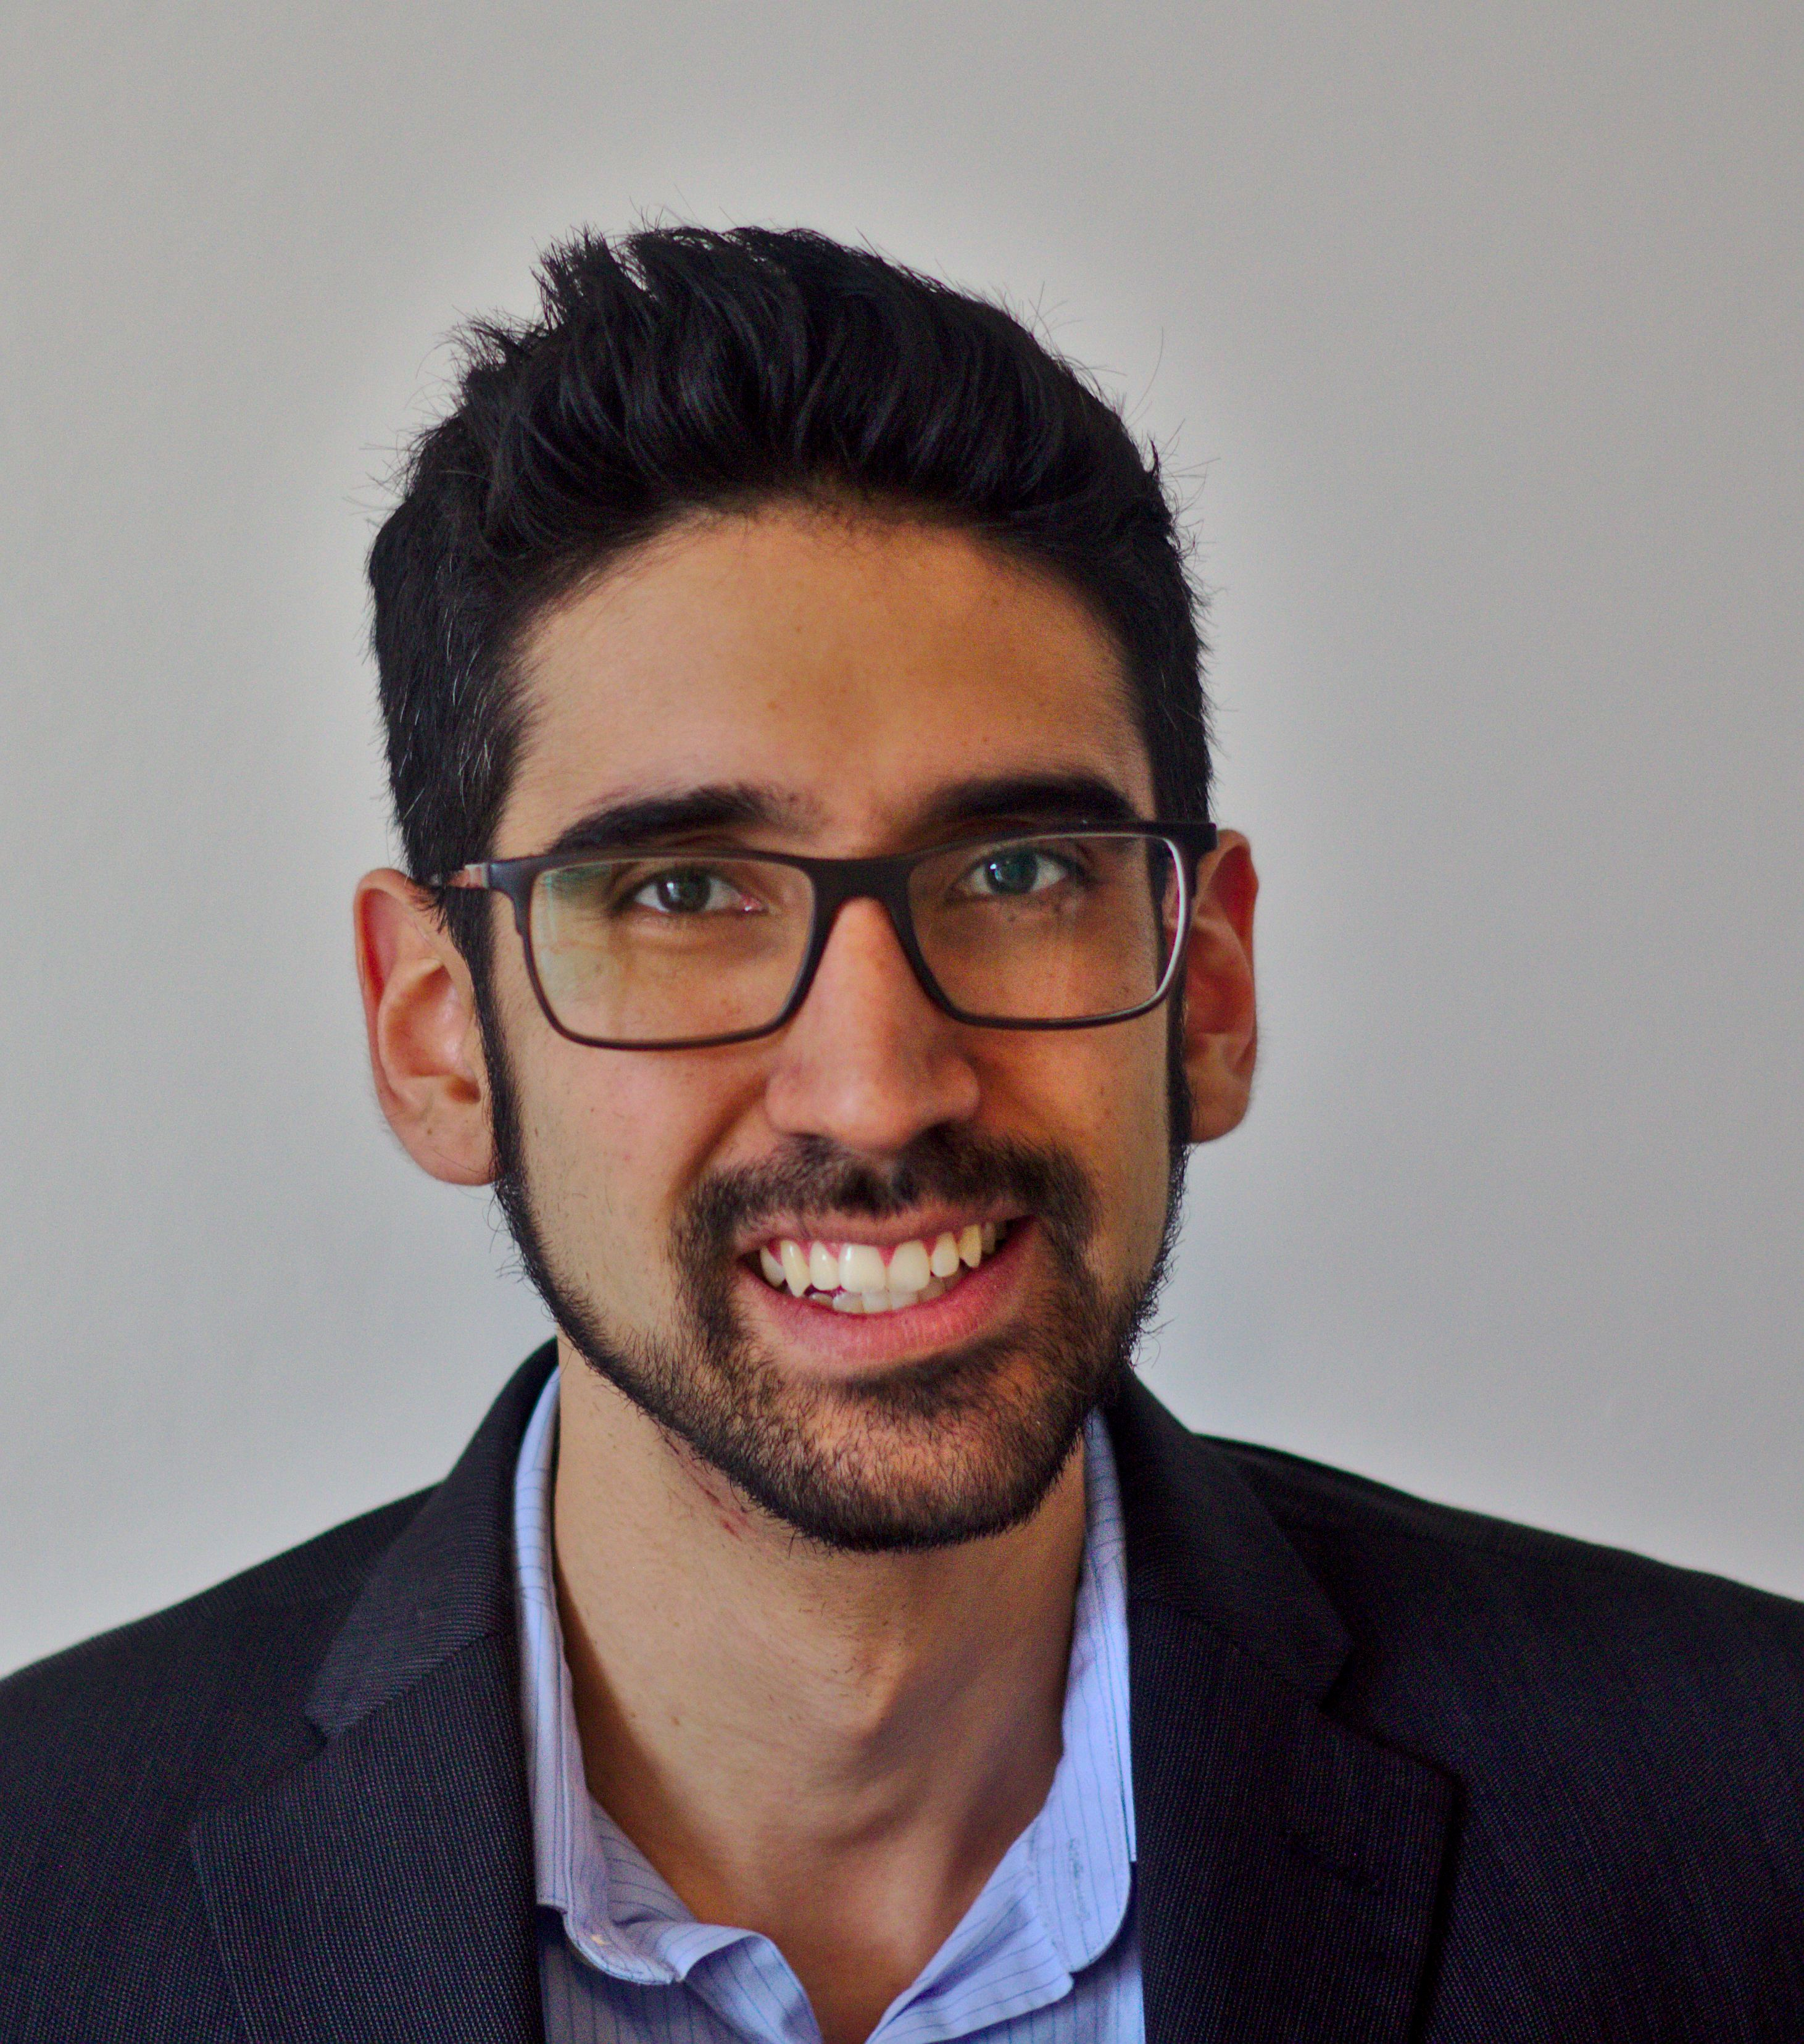
\includegraphics[width=0.19\textwidth]{cv_picture.jpg}}
\end{wrapfigure}

\MyName{Aníbal Sigüenza Torres}
{
	{\raggedleft{Date of birth: 06/06/1992\\
    			Paul-Hindemith-Allee 4, 80939 München\\
                \href{mailto:anibal.siguenza1@gmail.com}			{anibal.siguenza1@gmail.com}\\
                +49 017621428384\\
    			}
    }
}

%\begin{flushright}
%    \href{mailto:anibal.siguenza1@gmail.com}{anibal.siguenza1@gmail.com}
%\end{flushright}

\sepspace

%%% Personal details
%%% ------------------------------------------------------------

\NewPart{Professional Objective}{}

\par
I want to develop myself in a technology business area solving complex problems efficiently and creatively, with the use of science and technology. 


%%% Education
%%% ------------------------------------------------------------
\NewPart{Education}{}

\EducationEntry{M.Sc. Computational Science and Engineering (CSE)}{2016-2018}{Technical University of Munich (TUM) in Munich, Germany}{Currently studying.}
\sepspace

\EducationEntry{B.Sc. Engineering Physics}{2010-2015}{Monterrey Technological Institute in Monterrey, Mexico}{Final score of 94/100.}
\sepspace

\EducationEntry{Exchange Semester}{Aug-Dec 2014}{Victoria University in Melbourne, Australia}{Final average of High Distinction.}
\sepspace

%\EducationEntry{High Level Mathematics}{2008-2010}{International Baccalaureate at Monterrey Technological Institute CCM}{Final score of 5/7.}

%%% Work experience
%%% ------------------------------------------------------------
\NewPart{Work and Academic experience}{}

\EducationEntry{Intern Programming and Thermal Engineer}{Oct 2017 - Sept 2017}{Intel Deutschland GmbH}{While studying my master I worked in the simulation group for Intel iCDG. Where we did thermal simulations for improving robustness of semiconductor packages.}
\sepspace

\EducationEntry{Researcher Assistant}{Jan 2016 - Jun 2016}{Institute of Research in Applied  Math and Systems at UNAM University}{I collaborated with Phd. Gibran Puentes-Pineda in deep machine learning applied to video processing systems. The programming language in the project was Python with Theano library. The work was developed in a Linux platform. }
\sepspace

\EducationEntry{Optics Researcher}{Jan 2014-Dec 2015}{Photonics and Mathematical Optics Group at Tecnológico de Monterrey}{In this experience I worked with Phd. Julio Gutierrez, leader of the research group, in finding \href{https://www.osapublishing.org/josaa/abstract.cfm?uri=josaa-33-5-832}{ \textit{Creation Operators for Cartesian and Circular beam}}, title of the article we published in the Journal of the Optical Society of America A.}
\sepspace

\EducationEntry{Programmer Assistant}{Summers 2012 and 2013}{Stockware S.A. de C.V. inc., Full-time}{In this project we implemented and improved the security software code working in Powerbuilder language. A new protection method for the company which allows the remote control of the licensing was obtained.}
\sepspace

%\EducationEntry{Laboratory Instructor}{Jan-May 2013, Jan-May 2014 and Jan-May 2015}{Monterrey Technological Institute, Part-time}{I led the physics laboratory, complement to the engineering class Physics II. I taught physics concepts with experiments and tutorials. }
%\sepspace

%\iffalse %para cortar la página dos
%%% Skills
%%% ------------------------------------------------------------
\NewPart{Skills}{}

\SkillsEntry{Languages}{Spanish (First language), English (fluent), German (intermediate)}
\SkillsEntry{Software}{C++, MPI, Python, \textsc{Matlab}, MS Office}
\SkillsEntry{Professional}{Scientific computing, HPC, 	Computational Modeling, Physics,  Engineering}
\SkillsEntry{Personal}{Teaching, Autodidact, Teamwork, Leadership}


%%% Extracurricular Activities
%%% ------------------------------------------------------------
\NewPart{Extracurricular Activities}{}

% \extraAct{Math tutoring}{Aug 2010-May 2012}{Math and Physics Department at ITESM CMM}{As part of my Scholarship service I was in charge of giving Math tutoring for students.}
% \sepspace

% \extraAct{Math and Physics Teacher}{Summer 2012}{Copilco Community Center}{As part of my Social service I was in charge of giving the classes of Physics and Math to high school students.}
% \sepspace

\extraAct{Subcapitan}{2012-2014}{Ultimate Frisbee Monterrey Technological Institute Team}{I was subcapitan for the ultimate Frisbee team. I was in charge of giving the trainings and leading the team in the competitions.}  
\sepspace

\extraAct{Treasurer}{Aug 2010-Aug 2011}{IDeaS Student Sustainable Engineering Society}{I was in charge of the capital management for the student society IdeAS. I controlled the cash flow and the general accounting.}
\sepspace

\extraAct{Lead Acoustic Guitarist}{Aug 2007-May 2012}{Music Contemporary Orchestra ITESM CCM}{I was the guitarist of a small orchestra for the university. We had numerous presentations all over Mexico City representing the university.}
\sepspace



%%% Awards
%%% ------------------------------------------------------------
\NewPart{Awards}{}

\extraAct{CONACYT-DAAD 2016 Scholarship}{}{CONACYT $\&$ DAAD}{I was granted with economical support from Mexican and German government to study the CSE master program.}
\sepspace

\extraAct{Honor Academic Scholarship May 2010}{}{Monterrey Technological Institute Mexico City Campus}{I was granted with tuition and fees support to study my B.Sc degree for academic excellence.}
\sepspace

\extraAct{GARA program}{}{Monterrey Technological Institute Mexico City Campus}{I got a recognition for my participation in the GARA program of high performance students during my B.Sc degree.}
\sepspace

\extraAct{Academic excellence in semester Aug-Dic 2010 }{}{Monterrey Technological Institute Mexico City Campus}{I was recognized for obtaining an average of 95 or higher in an academic semester during my B.Sc degree.}
\sepspace

\extraAct{First place in Song Festival 2011}{}{Monterrey Technological Institute Mexico City Campus}{Our band won the first place in the composition contest for the best original song.}
\sepspace
%\fi  %para cortar página dos

\end{document}
